\section{Sensordaten aus Simulator CoppeliaSim}
Insgesamt wurden vier Routen über 20 Zyklen jeweils zwei mal erfasst.
Einmal für Trainingsdaten und einmal für Testdaten, wobei die letzten fünf Zyklen der
Trainingsdaten als Validationsmenge genutzt werden, die außerdem zur Feature-Auswahl genutzt wird.
Dabei wurden alle 50 ms die xyz-, Koordinaten, Accelerometerdaten und Gyroskopdaten erfasst, sowie Lichtintensität und Metadaten.
Zu den Metadaten gehören Zeitstempel, Beschriftung des Routenabschnitts und Beschriftung des derzeitigen Zyklusses.
Ein Zyklus ist der vollständige Umlauf einer Route.
\newpage
Abbildung \ref{fig:simple_square_labeled} zeigt eine der vier Routen \glqq simple\_square\grqq.
Jede Route ist mit Markierungen für Zyklen und Standorte ausgestattet.
Die Zyklusmarkierung wird genutzt, um die Datensätze mit dem derzeitigen Zyklus zu beschriften.
Jedes mal, wenn die Sensorenbox diese Markierung überschreitet, wird der Zähler für den Zyklus inkrementiert.
Die Standortmarkierung wird genutzt, um die Datensätze mit dem derzeitigen Routenabschnitt zu beschriften.
Jedes mal, wenn die Sensorenbox diese Markierung überschreitet, wird der derzeitige Wert für den Routenabschnitt auf den Wert der Markierung gesetzt.
Dabei werden alle aufgenommenen Datensätze immer mit dem derzeitigen Wert für den Routenabschnitt markiert.
\begin{figure}[h!]
    \centering
    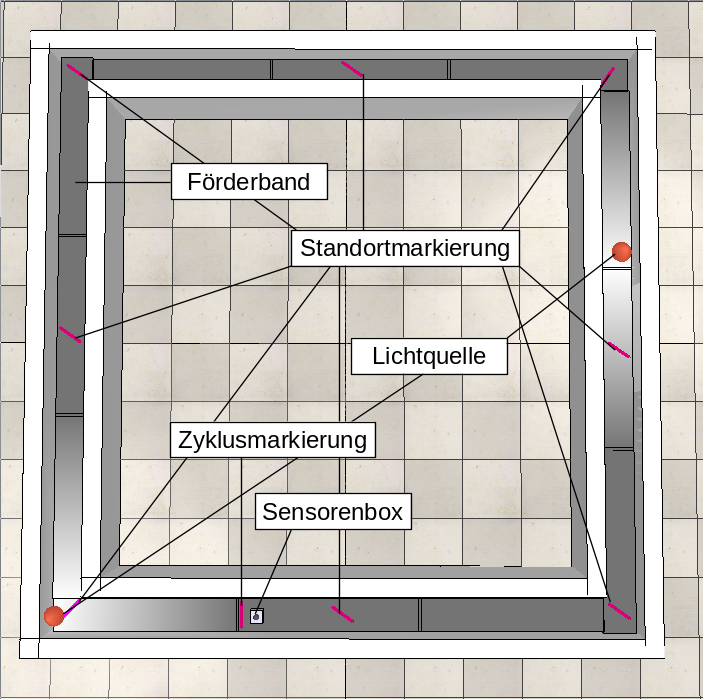
\includegraphics[width=\linewidth]{images/simple_square_labeled.png}
    \caption{Modell der Route \glqq simple\_square\grqq\ in CoppeliaSim mit Beschriftungen.}
    \label{fig:simple_square_labeled}
\end{figure}
\newpage
Neben \glqq simple\_square \grqq\ gibt es noch drei weitere Routen (siehe Abbildungen \ref{fig:long_rectangle}, \ref{fig:rectangle_with_ramp} und \ref{fig:many_corners}).
Die Route \glqq long\_rectangle \grqq\ weist lange Pfade mit wenig Änderungen auf.
Die Route \glqq rectangle\_with\_ramp \grqq\ besitzt zusätzlich zwei Rampen, wodurch Höhenunterschiede simuliert werden.
Die Route \glqq many\_corners \grqq\ ist sehr komplex und hat viele verschiedene Standorte.
Die Förderbänder können verschiedene Geschwindigkeiten haben mit sowohl abrupten Übergangen, als auch fließenden Übergängen zueinander.
\newline
\newline
Je nach Enkodierungsart (siehe Kapitel \ref{sec:model_location_encoding}) müssen die Knoten und Kanten, dieses zyklischen Graphen, als Standorte enkodiert werden.
Als Knoten wird die Menge der Datensätze bezeichnet, die sich in einem Umkreis des ersten Datensatzes befinden, der mit einem Standort in der Simulation markiert wurde.
Dadurch gibt es Datensätze, die zwar in der Simulation mit diesem Standort markiert wurden, aber nicht innerhalb des Umkreises von dem ersten Datensatz liegen
und somit zu diesen Knoten gehören.
Die Knoten werden mit dem Wert der Standortbeschriftung beschriftet.
Die übrigen Datensätze werden entweder als unbekannten Standort beschriftet oder erhalten einen Standortwert, der die Beziehung der Kante zwischen zwei Knoten enkodiert,
aber nicht in der Simulation markiert wurde.